\documentclass[11pt]{amsart}
\usepackage{geometry}                % See geometry.pdf to learn the layout options. There are lots.
\geometry{letterpaper}                   % ... or a4paper or a5paper or ... 
%\geometry{landscape}                % Activate for for rotated page geometry
%\usepackage[parfill]{parskip}    % Activate to begin paragraphs with an empty line rather than an indent
\usepackage{graphicx}
\usepackage{amssymb}
\usepackage{epstopdf}
\usepackage[usenames,dvipsnames]{color}
\usepackage{fancyvrb}
\usepackage{listings}
\usepackage{booktabs,footmisc}
\usepackage{hyperref}
\usepackage[all]{hypcap}

\usepackage{topcapt}


 
% include the lines below to use a nicer fixed-width font than the default one
 
\lstset{fancyvrb=true}
\lstset{
	basicstyle=\small\tt,
	identifierstyle=,
	commentstyle=\color{Bittersweet},
	stringstyle=\color{red},
	showstringspaces=false,
	tabsize=3,
	captionpos=b,
	xleftmargin=2em
%	numberstyle=\tiny
	%stepnumber=4
	}
\DeclareGraphicsRule{.tif}{png}{.png}{`convert #1 `dirname #1`/`basename #1 .tif`.png}

\title{Data Collection for Repast Simphony Java and ReLogo}
\author{Nick Collier - Repast Development Team}
%\date{\today}                                           % Activate to display a given date or no date

\begin{document} 
\maketitle
\setcounter{section}{-1}

\section{Before We Get Started}
This document is an introduction to the data collection system introduced in Repast Simphony 2.0 Final. It assumes a basic familiarity with Repast Simphony and / or ReLogo and is intended primarily for those moving from Repast Simphony 2.0 Beta to 2.0 Final. If you do not have any experience with Repast Simphony, please read the Repast Java and / or the ReLogo Getting Started tutorials.

\section{Overview}
Repast Simphony 2.0 Final (RS) records data from data sources. A wizard can be used to define data sources or you can create them yourself. Data sources come in two flavors Aggregate and Non- Aggregate. Aggregate data sources receive a collection of objects (agents, for example) and typically return some aggregate value calculated over all the objects. For example, an aggregate data source might call a method on each object and return the maximum value. A non-aggregate data source takes a single object (e.g. a single agent) and returns a value. For example, a non-aggregate data source might call a method on an agent and return the result of that method call. Note that RS will take care of which agents and objects to pass to which data source and perform the actual data collection. You just need to define the data source(s). For convenience, data sources are grouped into named data sets. A data set is a collection of data sources. 

Once a data set is defined, RS will record the data produced by the data set's data sources. However, the recorded data will not be written to a file or displayed in a chart. For that to occur, you must define a data sink. A data sink takes the data produced by data sources and writes them to a file, the console or displays them in a chart. The same data set can be connected to multiple data sinks. 

\section{Defining Data Sources and Data Sets}
Data collection is set up in Repast Simphony by defining the data sets and data sources described above. To create a data set, right click on the Data Sets node in the scenario tree and select "Add Data Set". You should a dialog like that in fig.~\ref{fig:ds1}. Here you can name the data set with a unique id and choose whether the data set will record aggregate or non-aggregate data. 

\begin{figure}[h]
\begin{center}
\vspace{.2in}
\centerline {
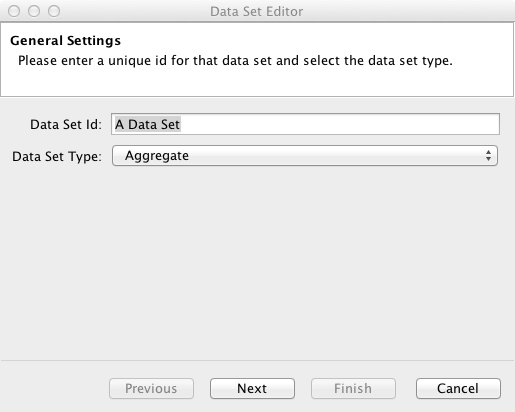
\includegraphics[width=4in]{images/ds_wizard_1.png}
}
\caption{Data Set Editor 1}
\label{fig:ds1}
\end{center}
\end{figure}

In the next step (click Next), you can define the data sources from which data will be recorded. In the data source step there are three different tabs you can choose from (see fig.~\ref{fig:ds2}).

The first tab "Standard Sources" is common to both types. Here you can select whether you want the current tick count, run number and / or random seed included in the data set. Click on a check box to add / remove one of the standard data sources.

\begin{figure}[h]
\begin{center}
\vspace{.2in}
\centerline {
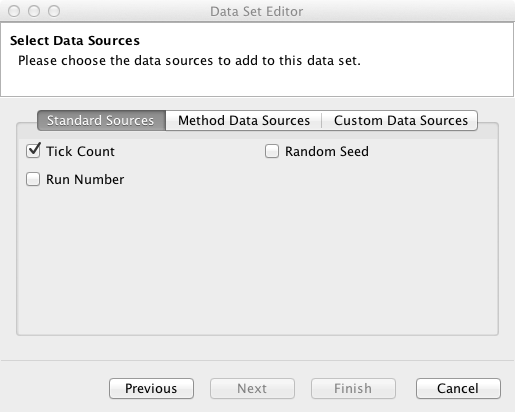
\includegraphics[width=4in]{images/ds_wizard_2.png}
}
\caption{Data Source Step}
\label{fig:ds2}
\end{center}
\end{figure}

The remaining two tabs function differently depending on the data set type (aggregate or non-) and are described below.

\subsection{Aggregate Data Sources}
For an aggregate data set, the method data source tab allows you to define a data source that calls a method on each of the agents (objects) of a specified type and then perform an aggregate operation on the results of those method calls. For example, if your model contains person agents, each of which have a getAge() method that returns the agent's age, you can create an aggregate data source to record the mean, maximum, and minimum age. 

To add an aggregate Method Data Source, click the "Add" button (see fig.~\ref{fig:agg_method}). A new row in the method data source table will be added. The type of agent you want to record data from can be selected by double clicking on the cell in the Agent Type column. The method to call on each of object of that type can be selected by double clicking on the cell in the Method column. The operation to apply to the results of the method calls can be selected by double clicking on the cell in the Aggregate Operation column. Note that boolean operations can be summed, averaged, and so forth. True is equal to 1 and false is equal to 0. You will also need to provide a name for the data source by double clicking and typing a name in the cell in the  Source Name column. 

An additional aggregate operation is provided that does not require a method. This "Count" operation will return the current number of agents of the specified type in the simulation. In the example in  fig.~\ref{fig:agg_method}, the Human Count data source will return the current number of "Human" agents whenever it is called. By selecting the "Count" operation the Method column cell with be set to a "N/A" (non-applicable) value indicating that the Count operation doesn't require a method call.


\begin{figure}[h]
\begin{center}
\vspace{.2in}
\centerline {
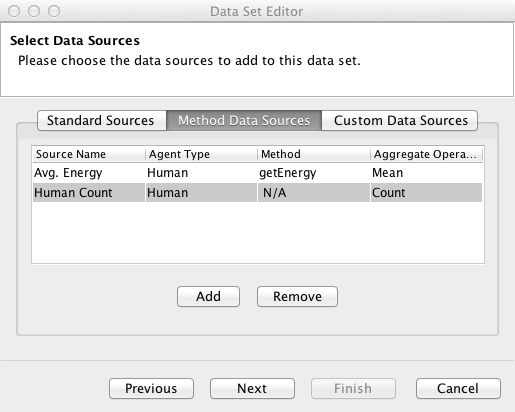
\includegraphics[width=4in]{images/agg_method.png}
}
\caption{Aggregate Method Data Sources}
\label{fig:agg_method}
\end{center}
\end{figure}

The Custom Data Sources tab (see fig.~\ref{fig:custom_ds}) allows you to specify your own custom data sources. Custom data sources are defined with the fully qualified name of a class that implements the repast.simphon.data2.AggregateDataSource interface. Type the name of the implementing class into the text box next to the "Add" button, then click the "Add" button. The new data source should appear in the list below the text box. More information on the AggregateDataSource interface can be found in the javadoc reference documentation.

\begin{figure}[h]
\begin{center}
\vspace{.2in}
\centerline {
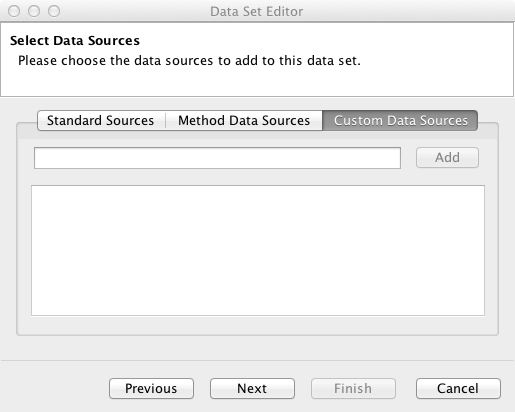
\includegraphics[width=4in]{images/custom_ds.png}
}
\caption{Custom Data Sources}
\label{fig:custom_ds}
\end{center}
\end{figure}

\subsection{Non-Aggregate Data Sources}
For a non-aggregate data set, the method data source tab (see fig.~\ref{fig:non-agg_method}) allows you to define data sources that call a method on an individual agent type and returns a result for each agent of that type. Unlike, the aggregate data source, no aggregate operation will be performed. The result of each call will be recorded. If you wanted to record the age or energy of an agent of a certain type, you could do that here.

To define a non-aggregate method data source, select the source class in the Source Class combo box and then click "Add" to add a new row to the method data source table. You can chose which methods to call by double clicking on the cell in the Method column. A default name will be supplied in the cell in Data Source Name column, but this is also editable by double clicking on that cell. Note on a single source class can be used, that is, all the method data sources need to be method calls on that selected class. 

\begin{figure}[h]
\begin{center}
\vspace{.2in}
\centerline {
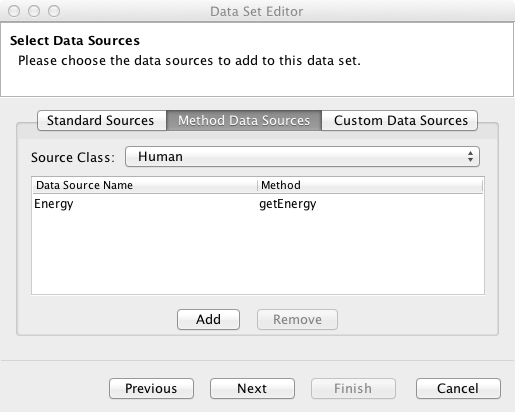
\includegraphics[width=4in]{images/non-agg_method.png}
}
\caption{Aggregate Method Data Sources}
\label{fig:non-agg_method}
\end{center}
\end{figure}

Custom data sources for non-aggregate data sets work the same way as aggregate data sets described above. However, the class must implement \\repast.simphony.data2.NonAggregateDataSource. 

Once you've defined your data sources, you can click "Next" and define when you want your data to be recorded. Click "Finish" to add the data set (and its data sources) to your scenario. Don't forget to save the scenario after adding new data sets.

\section{Writing Data}
Once the data set(s) have been defined, RS will record from the data sources in those data sets. RS can write data to both a file and the console. File output will write the recorded data out to a file. Console output will show up in Eclipse�s console tab and can be useful for debugging. 

To write data to a file, we need to define a file sink. To create a file sink right click "Text Sinks" in the Scenario Tree and click "Add File Sink". You should see a dialog like that in fig.~\ref{fig:fs}. The first step is to select the data set from any data sets you have created and then select the data sources you wish to record. You can select the data set using the Data Set ID combo box. Once you have selected the data set, you should see a list of the data sources in that data set in the list box on the left hand side. Select the ones you wish to write to a file and click the right arrow to move them over to the list of data sources to be written. You can change the order in which they will be written using the up and down arrows. 

\begin{figure}[h]
\begin{center}
\vspace{.2in}
\centerline {
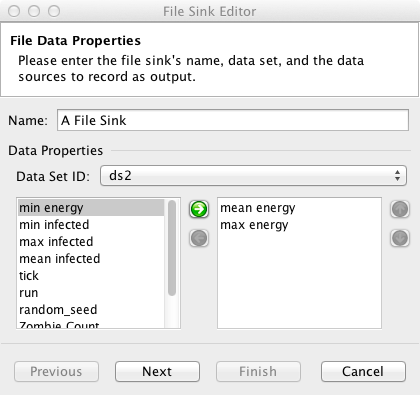
\includegraphics[width=4in]{images/fs1.png}
}
\caption{File Sink Dialog}
\label{fig:fs}
\end{center}
\end{figure}


\begin{figure}[h]
\begin{center}
\vspace{.2in}
\centerline {
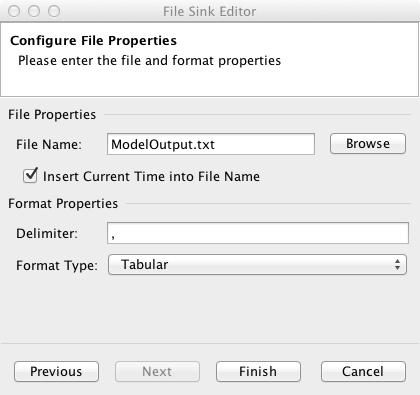
\includegraphics[width=4in]{images/fs2.png}
}
\caption{File Sink Dialog 2}
\label{fig:fs2}
\end{center}
\end{figure}



Once you've selected the data sources you wish to record, click Next to define the file properties (see fig.~\ref{fig:fs2}). The file name specifies the name of the file to write the data and you can specify whether or not to insert the current time into the file name. The delimiter string will be used use to separate the data entries. Data can be written in two formats. Tabular format records the data in typical spreadsheet type tabular format. Each data source will be a column in the table and the name of the data source will be the column header. For example,

\noindent\begin{minipage}[h]{\textwidth}
\vspace{.2in}
\lstset{language=java,caption=Tabular Output}
\begin{lstlisting}
"tick",	"Human Count",	"Zombie Count"
1.0,		199,				6
2.0,		199,				6
3.0,		198,				7
4.0,		195,				10
...
\end{lstlisting}
\vspace{.2in}
\end{minipage}

Line format writes the data out on a single line where the data source name is followed by a colon followed by the value. For example,

\noindent\begin{minipage}[h]{\textwidth}
\vspace{.2in}
\lstset{language=java,caption=Line Output}
\begin{lstlisting}
tick: 1.0, Human Count: 199, Zombie Count: 6
tick: 2.0, Human Count: 198, Zombie Count: 7
...
\end{lstlisting}
\vspace{.2in}
\end{minipage}

Click finish to add the file sink to the scenario and don't forget to save the scenario.

To define a console sink, click on the Text Sinks node in the scenario tree and select "Add Console Sink." The steps to define a console sink are nearly identical those used to define a file sink. You choose a data set, select the data sources from the data set, specify a delimiter and a format type. You can also enable / disable a console sink in the console sink wizard. This can be useful to enable a console sink for debugging and then disable it for production runs.

\subsection{Batch Runs}
Output during batch runs now consists of a single file. The file will automatically include the batch run number. For example,

\noindent\begin{minipage}[h]{\textwidth}
\vspace{.2in}
\lstset{language=java,caption=Batch Run Output}
\begin{lstlisting}
"run", "tick", "Human Count", "Zombie Count"
1, 1.0, 199, 6
1, 2.0, 199, 6
1, 3.0, 198, 7
...
2, 1.0, 199, 5
2, 2.0, 199, 5
2, 3.0, 198, 7

\end{lstlisting}
\vspace{.2in}
\end{minipage}

where "run" is the batch run number. A parameter mapping file will also be produced that describes what parameters were used for each run. For example,

\noindent\begin{minipage}[h]{\textwidth}
\vspace{.2in}
\lstset{language=java,caption=Batch Parameter Map Output}
\begin{lstlisting}
"run","randomSeed","human_count","zombie_count"
1, 1, 200, 5
2, 1, 200, 6
...
\end{lstlisting}
\vspace{.2in}
\end{minipage}

Here, run 1 was run with a random seed of 1, a human count of 200 and zombie count of 5. Run 2 was run with a random seed of 1, a human count of 200 and zombie count of 6. This mapping file will have the same name as the output file with "batch\_param\_map" inserted. So, ModelOutput.2012.Jan.27.14\_23\_34.txt will have a mapping file of ModelOutput.2012.Jan.27.14\_23\_34.batch\_param\_Map.txt.

\section{Charting Data}
RS allows you to create two different kinds of charts: time series and histograms. 

\subsection{Time Series}
To create a time series chart right click on the Charts node in the scenario tree and choose "Add Time Series Chart". You should see a dialog like that in fig.~\ref{fig:ts1}. Here you can type in a name for your chart and select the data set you wish to chart in the data set combo box. Note that the data set must contain a data source named "tick" in order to create a time series. The standard data source "current tick count" will provide this, but you can also create your own "tick" data source. The tick value will be the x-axis value. The next step will be different depending on the type (aggregate or non-) of data set you have chosen. 

\begin{figure}[h]
\begin{center}
\vspace{.2in}
\centerline {
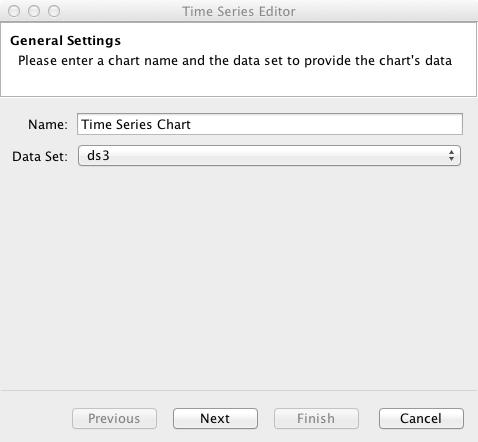
\includegraphics[width=4in]{images/ts1.png}
}
\caption{Time Series Editor}
\label{fig:ts1}
\end{center}
\end{figure}

When charting aggregate data, each  data source in the data set can become a series in the chart. The "Chart Data Properties" step (see fig.~\ref{fig:ts2}) allows you to select which of the data sources defined in the chosen data set will be displayed as series in the chart. You can select a data source for display in the chart by clicking the check box in the left most column of the table. You can also set the color of the displayed series by double clicking on the relevant cell in the color column. This will bring up a color selection dialog from which you can select a color for the series.

\begin{figure}[h]
\begin{center}
\vspace{.2in}
\centerline {
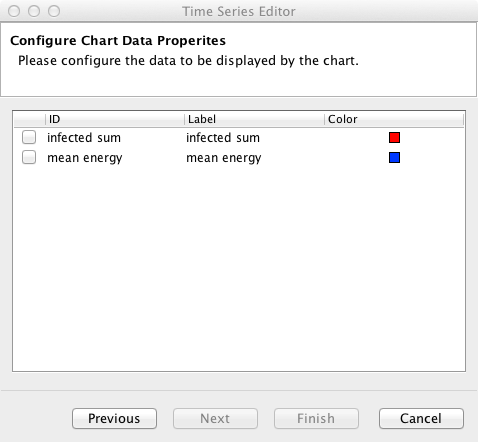
\includegraphics[width=4in]{images/ts2.png}
}
\caption{Time Series Aggregate Data Step}
\label{fig:ts2}
\end{center}
\end{figure}

When charting non-aggregate data, the series definition works differently. A non-aggregate data set  generates a row of data  or each object rather than aggregating the individual data into a single row. For example, you might have a data set that records the properties of each agent of some type in your model. When creating a time series from this type of data, each series will represent an individual agent and the y-value will be the value of some selected property of that agent. Consequently, in the data selection step (see fig.~\ref{fig:ts3}) for non-aggregate data, you need to select a data source that unique identifies that data as belonging to a particular agent, and also the data source to plot. For example, suppose you have a non-aggregate data set with data sources that record the amount of energy each agent in your model has, and the id of each agent. Each row of data then identifies the agent with an id and the amount of energy that agent has. You can plot the energy value of each agent by selecting the id data source in the Series ID combo box and the energy data source in the "Data To Display" combo box.

\begin{figure}[h]
\begin{center}
\vspace{.2in}
\centerline {
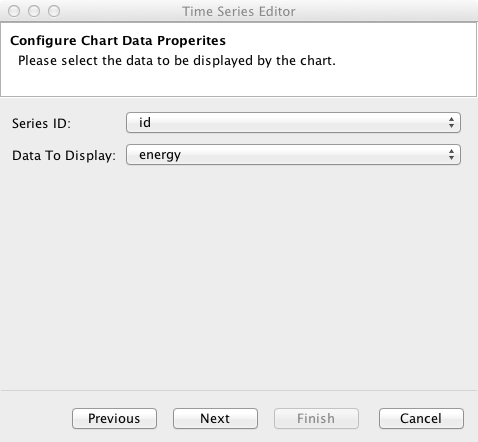
\includegraphics[width=4in]{images/ts3.png}
}
\caption{Time Series Non-Aggregate Data Step}
\label{fig:ts3}
\end{center}
\end{figure}

The final step (see fig.~\ref{fig:ts4}) in the time series wizard is the same regardless of the data set type. In this step, you can specify chart display properties such as the chart title and the x and y axis labels. You can also change the background and grid line colors of the chart by clicking their respective buttons. The chart gridlines can be turned on or off using the "Show Grid Lines" check box. Lastly, you can specify the x-axis range by using the "X-Axis Range" spinner. The x-axis range specifies how much of the x-axis you wish to see. For example, a range of 20 mean that only the last 20 ticks will be seen. A value of -1 indicates that the entire plot should be displayed. You can type a value directly into the spinner or use the up and down arrows to adjust the value.

\begin{figure}[h]
\begin{center}
\vspace{.2in}
\centerline {
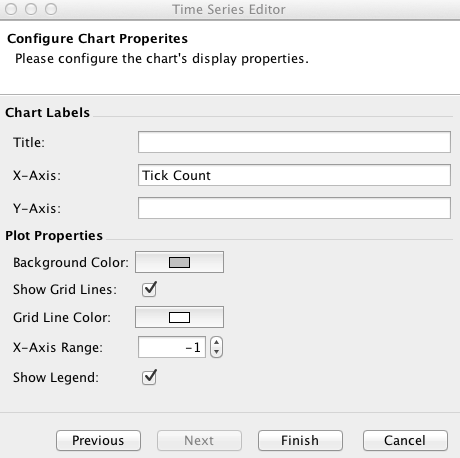
\includegraphics[width=4in]{images/ts4.png}
}
\caption{Timer Series Chart Properties Step}
\label{fig:ts4}
\end{center}
\end{figure}

Click finish to add the time series to the scenario. Don't forget to save the scenario.

\subsection{Histogram}
You can create a histogram chart by right clicking on the Charts node in the scenario tree and selecting "Add Histogram Chart". You should see a dialog like that in fig.~\ref{fig:h1}. A histogram chart works with non-aggregate data. It will histogram the data recorded by a single data source and then display it. For example, suppose you have a non-aggregate data set with a data source that records the amount of energy each agent in your model has. Each time data is recorded, that data set will record a number of energy values equal to the current number of agents in the model. The histogram chart will histogram these values and update the chart to display the histogram in a bar chart. Consequently, in the histogram data step you need to select the data set from which to get the data, and the specific data source to histogram.

\begin{figure}[h]
\begin{center}
\vspace{.2in}
\centerline {
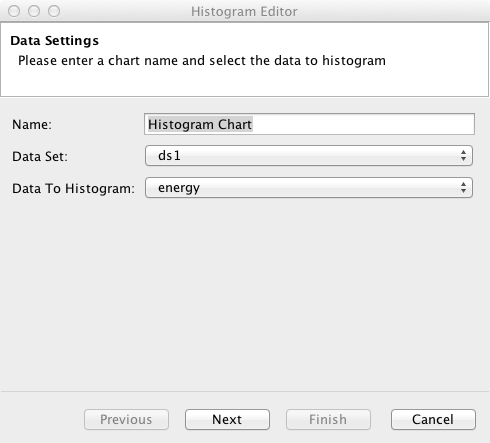
\includegraphics[width=4in]{images/h1.png}
}
\caption{Histogram Data Step}
\label{fig:h1}
\end{center}
\end{figure}

Once that is done, you can click next to move to the histogram properties step (see. fig.~\ref{fig:h2}). Here you select the number of bins in the histogram and the histogram type. If the type is dynamic then the histogram maximum and minimum values will update depending on the current data. If the type is static, then you need to provide the maximum and minimum values and choose how values outside that range are handled. The Out of Range options are:

\begin{itemize}
\item Ignore - out of range values will be ignored
\item Add to Min / Max Bins - items less than min will count in the minimum value bin and items greater than max will count in the maximum value bin
\item Display Values in Chart Subtitle - a chart subtitle will display overflow and underflow counts.
\end{itemize}

\begin{figure}[h]
\begin{center}
\vspace{.2in}
\centerline {
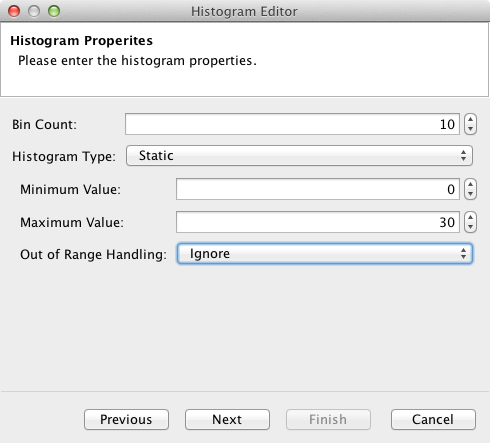
\includegraphics[width=4in]{images/h2.png}
}
\caption{Histogram Properties Step}
\label{fig:h2}
\end{center}
\end{figure}

The final step allows you to configure the charts properties (see fig.~\ref{fig:h3}). Here you can provide titles for the chart and the x- and y- axes. You can also set the color of the bars in the chart as well as the color of the background and grid lines. Click the respective buttons to set the color. Lastly, the gridlines can be turned on and off using the grid line checkbox.

Click finish to add the histogram to the scenario. Don't forget to save the scenario.


\begin{figure}[h]
\begin{center}
\vspace{.2in}
\centerline {
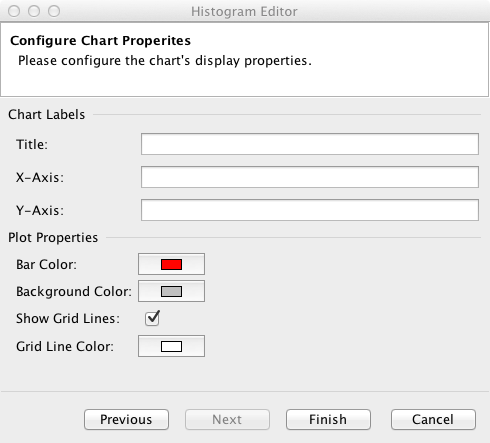
\includegraphics[width=4in]{images/h3.png}
}
\caption{Histogram Chart Properties Step}
\label{fig:h3}
\end{center}
\end{figure}



\end{document}  